125. \begin{figure}[ht!]
\center{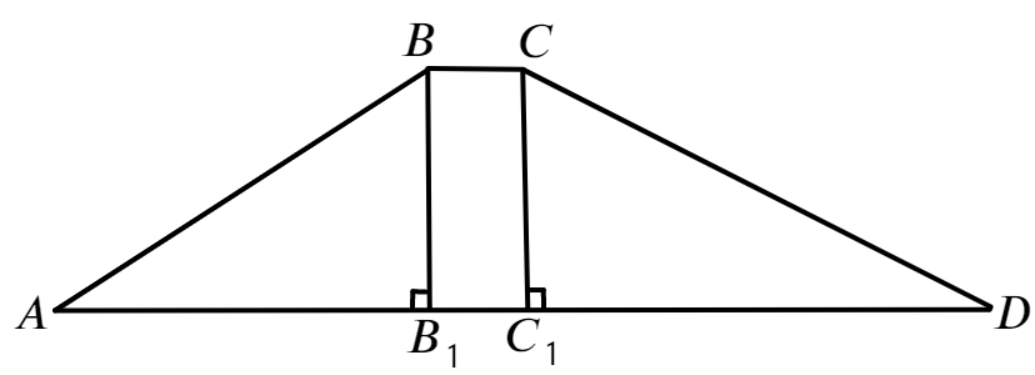
\includegraphics[scale=0.35]{g9-125.png}}
\end{figure}\\
Так как трапеция является описанной, суммы её противоположных сторон равны и $AB=CD=\cfrac{1+25}{2}=13.$ Опустим высоты $BB_1$ и $CC_1,$ тогда $AB_1=C_1D=\cfrac{25-1}{2}=12$ и по теореме Пифагора $BB_1=CC_1=\sqrt{13^2-12^2}=5,$ поэтому $S_{ABCD}=5\cdot\cfrac{1+25}{2}=65.$
ewpage
oindent
